\documentclass{article}
    % General document formatting
    \usepackage[margin=0.7in]{geometry}
    \usepackage[parfill]{parskip}
    \usepackage[utf8]{inputenc}
    \usepackage{amsmath}
    \usepackage{amssymb}
    \usepackage{tikz}
    \usepackage{fancyhdr}

\pagestyle{fancy}
\fancyhf{}
\rhead{Edgar Jacob Rivera Rios - A01184125}

\begin{document}
\section*{1.2.1}
(a) Show that $A \times (B \cap C) = (A \times B) \cap (A \times C)$
\begin{align*}
    (x, y) \in A \times (B \cap C) &\implies x \in A \wedge y \in (B \cap C)\\
    &\implies x \in A \wedge y \in B \wedge y \in C\\
    (x, y) \in (A \times B) \cap (A \times C)&\implies (x, y) \in (A \times B) \wedge (x, y) \in (A \times C)\\
    &\implies x \in A \wedge y \in B \wedge x \in A \wedge y \in C\\
    &\implies x \in A \wedge y \in B \wedge y \in C
\end{align*}
(b) Show that $A \times (B \cup C) = (A \times B) \cup (A \times C)$
\begin{align*}
    (x, y) \in A \times (B \cup C) &\implies x \in A \wedge y \in (B \cup C)\\
    &\implies x \in A \wedge (y \in B \vee y \in C)\\
    (x, y) \in (A \times B) \cup (A \times C)&\implies (x, y) \in (A \times B) \vee (x, y) \in (A \times C)\\
    &\implies (x \in A \wedge y \in B) \vee (x \in A \wedge y \in C)\\
    &\implies x \in A \wedge (y \in B \wedge y \in C)
\end{align*}

\section*{1.2.2}
(a) Consider the relations $R=\{ (1,7), (3,3), (13,11) \}$ and $S=\{ (1,1), (1,7), (3,11), (13,12), (15,1) \}$ over the positive integers. Identify $dom(R\cap S)$, $range(R\cap S)$, $dom(R\cup S)$, $range(R\cup S)$
\begin{equation*}
    dom(R\cap S) = \{ 1\}
\end{equation*}
\begin{equation*}
    range(R\cap S) = \{ 7\}
\end{equation*}
\begin{equation*}
    dom(R\cup S) = \{ 1, 3, 13, 15 \}
\end{equation*}
\begin{equation*}
    range(R\cup S) = \{ 7, 3, 11, 1, 12 \}
\end{equation*}
(b) In the same example, identify $join(R,S)$, $join(S,R)$, $S \circ R$, $R\circ S$, $R \circ R$, $S \circ S$.
\begin{equation*}
    join(R,S) = \{ (3,3,11) \}
\end{equation*}
\begin{equation*}
    join(S,R) = \{ (1, 1, 7), (15, 1, 1) \}
\end{equation*}
\begin{equation*}
    S \circ R = \{ (1,7), (15, 1) \}
\end{equation*}
\begin{equation*}
    R \circ S = \{ (3, 11) \}
\end{equation*}
\begin{equation*}
    R \circ R = \{ (3, 3) \}
\end{equation*}
\begin{equation*}
    S \circ S = \{ (1, 1), (1, 7), (15, 1), (15, 7) \}
\end{equation*}
(c) In the same example, identify $R(X)$ and $S(X)$ for $X=\{ 1, 3, 11 \}$ and $X=\emptyset$.
\begin{align*}
    X&=\{ 1, 3, 11 \} & X&=\emptyset\\
    R(X)&=\{(1,7), (3,3)\} & R(X) &=\emptyset\\
    S(X)&=\{ (1,1), (1,7), (3,11)\} & S(X) &=\emptyset\\
\end{align*}
(d) Explain how to carry out composition by means of join and projection.\\
Composition is the result of first applying the $join$ and thenn ussing the $projection$ to eliminate the common item

\section*{1.2.3}
(a) Show that R is reflexive over $A$ iff $I_A \subseteq R$. Here $I_A$ is the identity relation over $A$, defined in an exercise in Sect. 2.1.3.
\begin{align*}
    R\ is\ reflexive\ in\ A &= \forall x \in A: xRx\\
    I_A &= \{(a,a): a \in A\}\\
    I_A &\subseteq R\\
    \forall a \in A &\implies \exists (a, a) \in I_A\\
    I_A \subseteq R &\implies \exists(a,a) \in R\\
    &\implies R\ is\ reflexive\ on\ A
\end{align*}
(b) Show that the converse of a relation $R$ that is reflexive over a set $A$ is also reflexive over $A$.
\begin{align*}
    R\ is\ reflexive\ over\ A &= \forall x \in A: xRx\\
    R^{-1} &= \{(a, b): (b, a) \in R\}\\
    R = \{(a, b): a = b \wedge\ a, b \in A\} &\implies (a, b) = (b, a)\\
    &\implies R^{-1} = R\\
    &\implies R^{-1}\ is\ reflexive\ over\ A
\end{align*}
(c) Show that R is transitive iff $R \circ R \subseteq R$.
\begin{align*}
    R\ is\ transitive &\iff R \circ R \subseteq R\\
    R \circ R &= \{(a, c): aRb \wedge bRc\}\\
    R \circ R \subseteq R &\implies (a, c) \in R\\
    &\implies R(R(a,b), c) = R(a, R(b, c))
\end{align*}
\newpage

\section*{1.2.4}
(a) Show that the following three conditions are equivalent: (i) $R$ is symmetric, (ii) $R \subseteq R^{-1}$ , (iii) $R = R^{-1}$.
\begin{align*}
    R\ is\ symetric \equiv R &\subseteq R^{-1} \equiv R = R^{-1}\\
    R\ is\ symetric &= \forall(a,b) \in R \exists (b,a) \in R\\
    R \subseteq R^{-1} &\implies \forall (a,b) \in R, \exists (a, b) \in R^{-1}\\
    &\implies (a,b) = (b, a)\\
    &\implies R = R^{-1}\\
    R = R^{-1}&\implies \forall (a,b) \in R, \exists (a, b) \in R^{-1}= \forall(a,b) \in R \exists (b,a) \in R\\
    &\therefore R\ is\ symetric \equiv R \subseteq R^{-1} \equiv R = R^{-1}
\end{align*}
(b) Show that if $R$ is reflexive over $A$ and also transitive, then the relation $S$ defined by $(a,b) \in S$ iff both $(a,b) \in R$ and $(b,a) \in R$ is an equivalence relation.
\begin{align*}
    reflexive &= (a, a) \in R \forall a \in A \\
    S &= \{(a, b):(a,b) \in R \wedge (b,a) \in R \}\\
    (a,b) \in R \wedge (b,a) \in R &\implies a = b\\
    &\implies S\ is\ equivalent
\end{align*}
(c) Enumerate all the partitions of $A=\{ 1, 2, 3 \}$ and draw a Hasse diagram for them under fineness.
\begin{align*}
    Partition(A) =\{&\{\{1\}, \{2\}, \{3\}\},\\
    &\{\{1, 2\},\{3\}\},\\
    &\{\{1, 3\},\{2\}\},\\
    &\{\{2, 3\},\{1\}\},\\
    &\{\{1, 2, 3\}\}\}
\end{align*}
\begin{center}
    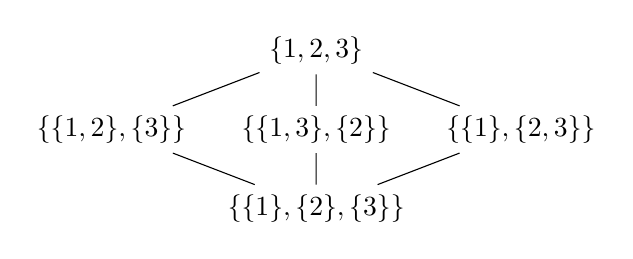
\begin{tikzpicture}[xscale=1.3, yscale=1]
        \node (bottom) at (0,0) {$\{\{1\}, \{2\}, \{3\}\}$};
        \node (middle) at (0, 1) {$\{\{1, 3\},\{2\}\}$};
        \node (middleleft) at (-2,1) {$\{\{1, 2\},\{3\}\}$};
        \node (middleright) at (2,1) {$\{\{1\},\{2, 3\}\}$};
        \node [above of=middle] (top)  {$\{1, 2, 3\}$};
        \draw (bottom) -- (middleleft) -- (top) -- (middle) -- (bottom) -- (middleright) -- (top);
    \end{tikzpicture}
\end{center}

\section*{1.2.5}
Let $R$ be any transitive relation over a set $A$. Define $S$ over $A$ by putting $(a,b) \in S$ iff either $a = b$ or both $(a,b) \in R$ and $\neg (b,a) \in R$. Show that $S$ partially orders $A$.
\begin{align*}
    Partial\ order &= reflexive,\ transitive\ and\ antisymmetric\\
    reflexive &= (a, a) \in R \forall a \in A \\
    %transitive &= \\
    antisymmetric &= (a,b) \in R \wedge (b,a) \notin R\\
    S &= \{(a, b): a = b \vee [(a,b) \in R \wedge (b,a) \notin R ]\}\\
    \{(a, b) : a = b\} &\implies S\ is\ reflexive\\
    \{(a, b) :(a,b) \in R \wedge (b,a) \notin R\} &\implies S\ is\ transitive\\
    &\implies S\ is\ antisymmetric
\end{align*}
\end{document}